\chapter{Physics objects definitions} % Main chapter title

\label{Chapter5} % Change X to a consecutive number; for referencing this chapter elsewhere, use \ref{ChapterX}

\fancyhead[LE,RO]{Chapter 5. \emph{Physics object definitions}} % Change X to a consecutive number; this is for the header on each page - perhaps a shortened title

The CMS detector is designed to efficiently reconstruct and identify interesting physics objects. The reconstruction procedure which takes as input the signals from all subdetectors and combines them to get physics objects is called \textit{particle flow} \cite{CMS:2009nxa}. This algorithm classifies all the objects into one of the following categories: charged hadrons, neutral hadrons, photons, electrons and muons. These are built from reconstructed tracks in the inner tracking system, energy deposits in the calorimeters and signals in the muon chambers, which are all combined to create a global event description. Additionally, a set of requirements is imposed on both input signals and reconstructed object in order to minimize the misidentification, e.g wrongly identifying electron as a jet. 
\par The following sections show electron and muon reconstruction procedures and identification criteria. Jet reconstruction procedure is then described together with necessary jet corrections and b-tagging algorithms. After the reconstruction of all other objects, missing transverse energy is computed as the imbalance of the vectorial sum of traverse momentum of all reconstructed particles.

%----------------------------------------------------------------------------------------
%	SECTION 1
%----------------------------------------------------------------------------------------

\section{Electrons}

Electrons in CMS are detected as a tracks in tracking system and an energy deposit in the electromagnetic calorimeter. Two different algorithms are used for electron reconstruction, \textit{tracker driven} seeding which is more suitable for low $p_T$ electrons and electrons inside jets and \textit{ECAL driven} seeding optimized for high $p_T$ isolated electrons. Both approaches take electromagnetic crystals with deposited energy and join them into \textit{clusters}. This process begins by identifying the cryistal with the highest energy deposit which becomes the seed for the cluster. An electron passing through the detector bends due to the magnetic field and interacts with the detector material emitting \textit{bremsstrahlung} photons. ECAL energy deposits from these photons are spread in $\phi$ direction in a very narrow $\eta$ range and combined with the existing cluster forming a \textit{supercluster}. Trajectories are reconstructed using modeling of electron energy loss in the detector material and fitted with a Gaussian Sum Filter (GSF) \cite{2005JPhG31N9A}.
\par The two approaches differ in the way they match ECAL superclusters and reconstructed tracks. Tracker driven algorithms use track from the tracking system and try to match it with the supercluster in the ECAL, while ECAL driven algorithms start from the superclusters.
Each electron candidate has to pass various quality criteria in order to maximize the probability of identifying the electron coming from the hard interaction, and reject electrons from jets or conversions. These selection criteria can be divided into three categories: identification, isolation and conversion rejection. Details on electron reconstruction and performance can be found in \cite{CMS:2010bta}.

%-----------------------------------
%	SUBSECTION 1.1
%-----------------------------------
\subsubsection*{Electron identification}
\label{sec:eleID}

The electron identification procedure first focuses on good matching between reconstructed track and supercluster, by imposing cuts on spatial distance $\Delta \eta$ and $\Delta \phi$ between the two. These variables are computed as absolute $\eta$ and $\phi$ distance between the supercluster and electron track extrapolated to the ECAL surface. Additionally, a cut is imposed on $\sigma_{i\eta i\eta}$ which is a measure of a shower shape spread in $\eta$ direction. This variable discriminates between energy deposits coming from electrons and photons, which are narrow, and jets, which are wide. Shower shape is defined as:
\begin{equation}
\sigma_{i\eta i\eta} = \sqrt{\frac{\sum_{i}^{5\times 5} w_i(\eta_i-\eta_{seed})^2\times \Delta \eta^2_{xtal} }{\sum_{i}^{5\times 5}}}
\end{equation}
where $i$ runs over all crystals in $5\times5$ block around the supercluster seed, $\eta_i-\eta_{seed}$ is the distance in number of crystals in $\eta$ direction between $i$-th crystal in supercluster and the seed crystal and $\Delta \eta_{xtal}$ is the average width of a single crystal. Each crystal is given a weight defined as $w_i=max(0,4.7+ln(E_i/E_{5\times5}))$, where $E_i$ is a single crystal energy, and $E_{5\times 5}$ is the sum of energy deposits inside a 5$\times$5 crystal block. 
Additional cut on the ratio between the energy deposits in the hadronic and electromagnetic calorimeter for electrons is used to discard the electron candidates with significant hadron activity.
\par Electrons coming from photon conversions are rejected by requiring a hit in every layer of the inner tracking system. Additionally, for each electron track a fit is performed trying to combine it with another electron track under the hypothesis that both electrons originate from a converted photon. Electron is selected only if this probability is sufficiently small. Electron compatibility with the primary vertex is estimated by looking at the impact parameters in both $xy$ and $z$ planes. Due to the gap in the electromagnetic calorimeter in 1.4442 $< |\eta| <$ 1.566, all electrons which have a supercluster position reconstructed in this range are rejected. A full list of identification criteria is summarized in Table \ref{tab:eleID}.
 \begin{table}[h]
\centering
  \caption{Summary of electron identification criteria used in this analysis.}
  \label{tab:eleID}
  \begin{tabular}{ l  c c}
      \hline
      \hline
      	Variable & Barrel & Endcap \\
      	\hline
    		$\Delta\eta$ $<$ &  0.004 & 0.005 \\
     	$\Delta\phi$ $<$ &  0.03 & 0.02 \\
     	$\sigma_{i\eta i\eta}$ $<$ & 0.01 & 0.03 \\
		$H/E$ $<$ & 0.12 & 0.10 \\
		$d_{xy}$ $<$ & 0.02 cm & 0.02 cm \\
		$d_{z}$ $<$  & 0.1 cm & 0.1 cm \\
		$(1/E - 1/p)$ $<$ & 0.05 & 0.05\\
		Missing hits  & 0 & 1 \\
		Vertex Fit Probability & $10^{-6}$ & $10^{-6}$ \\    	

      \hline
      \hline 
  \end{tabular}
\end{table}


%----------------------------------------------------------------------------------------
%	SECTION 2
%----------------------------------------------------------------------------------------

\section{Muons}

Muons in CMS are reconstructed by combining a reconstructed track inside the tracker(\textit{tracker track}) and a track in muon chambers (\textit{standalone muon track}). Individual track segments in the muon chambers are fitted using a Kalman filter technique \cite{Fruhwirth1987444}  in order to obtain a standalone muon track. As for electrons, two approaches are used for combining track from tracker and standalone track. 
\par \textit{The global muon reconstruction} approach uses a standalone muon track in the muon chambers and tries to find a matching tracker track by combining parameters of the two tracks by projecting it to the common surface. This \textit{outside-in} approach uses Kalman fitter technique to combine these two objects in an object called \textit{global muon}. Muon momentum is then determined from this global muon track using all available systems which shows improved precision in comparison to other approaches.  
\par The second approach for muon reconstruction is \textit{tracker muon reconstruction} which starts from tracks inside the tracker with $p_T>0.5$ GeV/c and total momentum $p>2.5$ GeV/c as potential muon candidates. Extrapolation is than performed to the muon chambers taking into account the magnetic field, Coulomb scattering in the material and other energy losses. \textit{Tracker moun} is found if at least one muon segment matches the extrapolated track. The efficiency of the \textit{Tracker muon} reconstruction is higher for low energy muons than the efficiency for the global muons, because only a single muon segment in the muon chambers is required. For high energy muons where there are more segments inside muon chambers, the \textit{global muon} algorithm is designed to have high efficiency. Detailed muon reconstruction procedure is shown in \cite{2012JInst7P0002T}.    

%-----------------------------------
%	SUBSECTION 2.1
%-----------------------------------

\subsubsection*{Muon identification}
\label{sec:muID}

In this analysis \textit{particle flow} muon identification selection is applied to the \textit{global muons}. A selection is applied in order to minimize misidentification of charged hadrons as muons, maximize the efficiency of muon identification inside jets and ensure good momentum measurement. Muons used in the analysis have $|\eta|<2.1$ and transverse momentum $p_T>30$ GeV with more than 5 hits in the inner tracker system and at least one hit in pixel detector. At least one good muon chamber hit is required and the \textit{global muon} track fit is required to have $\chi^2/ndof<10$. At least two segments in two different muon stations should be matched to a track in order to suppress muons from in-flight decays. Cosmic muons are rejected by applying cuts on the impact parameter with respect to the primary vertex, $|d_{xy}|<$0.2 cm and $|d_z|<$ 0.5 cm. Muon identification criteria are summarized in Table \ref{tab:muID}.

  \begin{table}[h]
\centering
  \caption{A summary of muon identification criteria.}
  \label{tab:muID}
  \begin{tabular}{ l  c c}
      \hline
      \hline
      	Variable & Requirement \\
      	\hline
    		number of pixel hits $>$ &  0 \\
     	number of inner tracker hits $>$ &  5 \\
     	$\chi^2/ndof$ $<$ & 10 \\
		number of muon hits $>$ & 0  \\
		chambers with matched segments $>$ & 1  \\		
		$d_{xy}$ $<$ & 0.2 cm \\
		$d_{z}$ $<$  & 0.5 cm \\
      \hline
      \hline 
  \end{tabular}
\end{table}
 

%-----------------------------------
%	SUBSECTION 2.2
%-----------------------------------

\section{Lepton isolation}
Leptons from W decays are in general expected to be well isolated from other particles in the final state. The degree of isolation is calculated using \textit{particle flow} approach by summing the transverse momenta contributions of particles around the lepton inside a specific cone. All charged particles as well as photons and neutral hadrons are considered if they have $p_T>$0.5 GeV. The cone used for determination of energy deposits is defined as $\Delta R = \sqrt{\Delta \phi^2+ \Delta \eta^2}$ around the lepton axis and isolation measure is defined as:
\begin{equation}
I_{PF}^{rel} = \frac{\sum p_T^{charged} + max(0, \sum E_T^{\gamma}+\sum E_T^{neutral}-0.5\sum E_T^{PU})}{p_T^l}
\end{equation}
where $\sum p_T^{charged}$ is the sum of the momenta of charged hadrons and $E_T^{\gamma} $ and $E_T^{neutral}$ are the sums of photon and neutral hadron momenta. $E_T^{PU}$ is the sum of the pile-up transverse energies from charged particles and is calculated as a sum of track transverse momenta not coming from the primary vertex inside the isolation cone. This is multiplied by the factor of 0.5, which corresponds approximately to the ratio of neutral to charged hadron production in the hadronization process of pile-up interactions. Selected muons are required to pass isolation cut $I_{rel}^{PF}<0.12$. On the other hand, if there is a requirement that there be no leptons in the event, the isolation cut is $I_{PF}^{rel}<0.2$. Electron isolation is computed in the very same way with cut of $I_{rel}^{PF}<0.1$ for selected electrons and $I_{rel}^{PF}<0.15$ for vetoed additional electrons.


%----------------------------------------------------------------------------------------
%	SECTION 3
%----------------------------------------------------------------------------------------

\section{Jets}

In high energy physics, a jet is a collimated group of hadrons which emerges as a result of quark or gluon fragmentation and hadronization process. Hadrons reconstructed in a particle detector need to be combined in order to form a jet and give information about the initial parton. A set of rules has to be created which define how to group particles and how to assign momentum to the jet. Usually this is done by summing the four-momentum of each particle in a jet.

%-----------------------------------
%	SUBSECTION 3.1
%-----------------------------------

\subsection{Jet algorithms}

Jet algorithms take into account the distance between particles and define rules to determine which particle belongs to what jet. The same jet algorithms should be applicable to both, experimental data and theoretical calculation.  Other important properties of jet algorithms are \textit{infrared safety} and \textit{collinear safety} which means if an event is modified by addition of soft emission of collinear splitting, the final number of hard jets will remain unchanged. These two properties together are called \textit{IRC safety}. IRC unsafe jet algorithms may break the cancellation of divergences by yielding one set of jets for tree-level splitting while loop diagrams lead to another, as shown if figure \ref{fig:jet_unsafe}, giving infinite cross-sections in the full calculations. Jet definitions, jet relation to partons and an overview of different jet algorithms are summarized in \cite{Salam:2009jx}.
\begin{figure}[htbp]
	\centering
		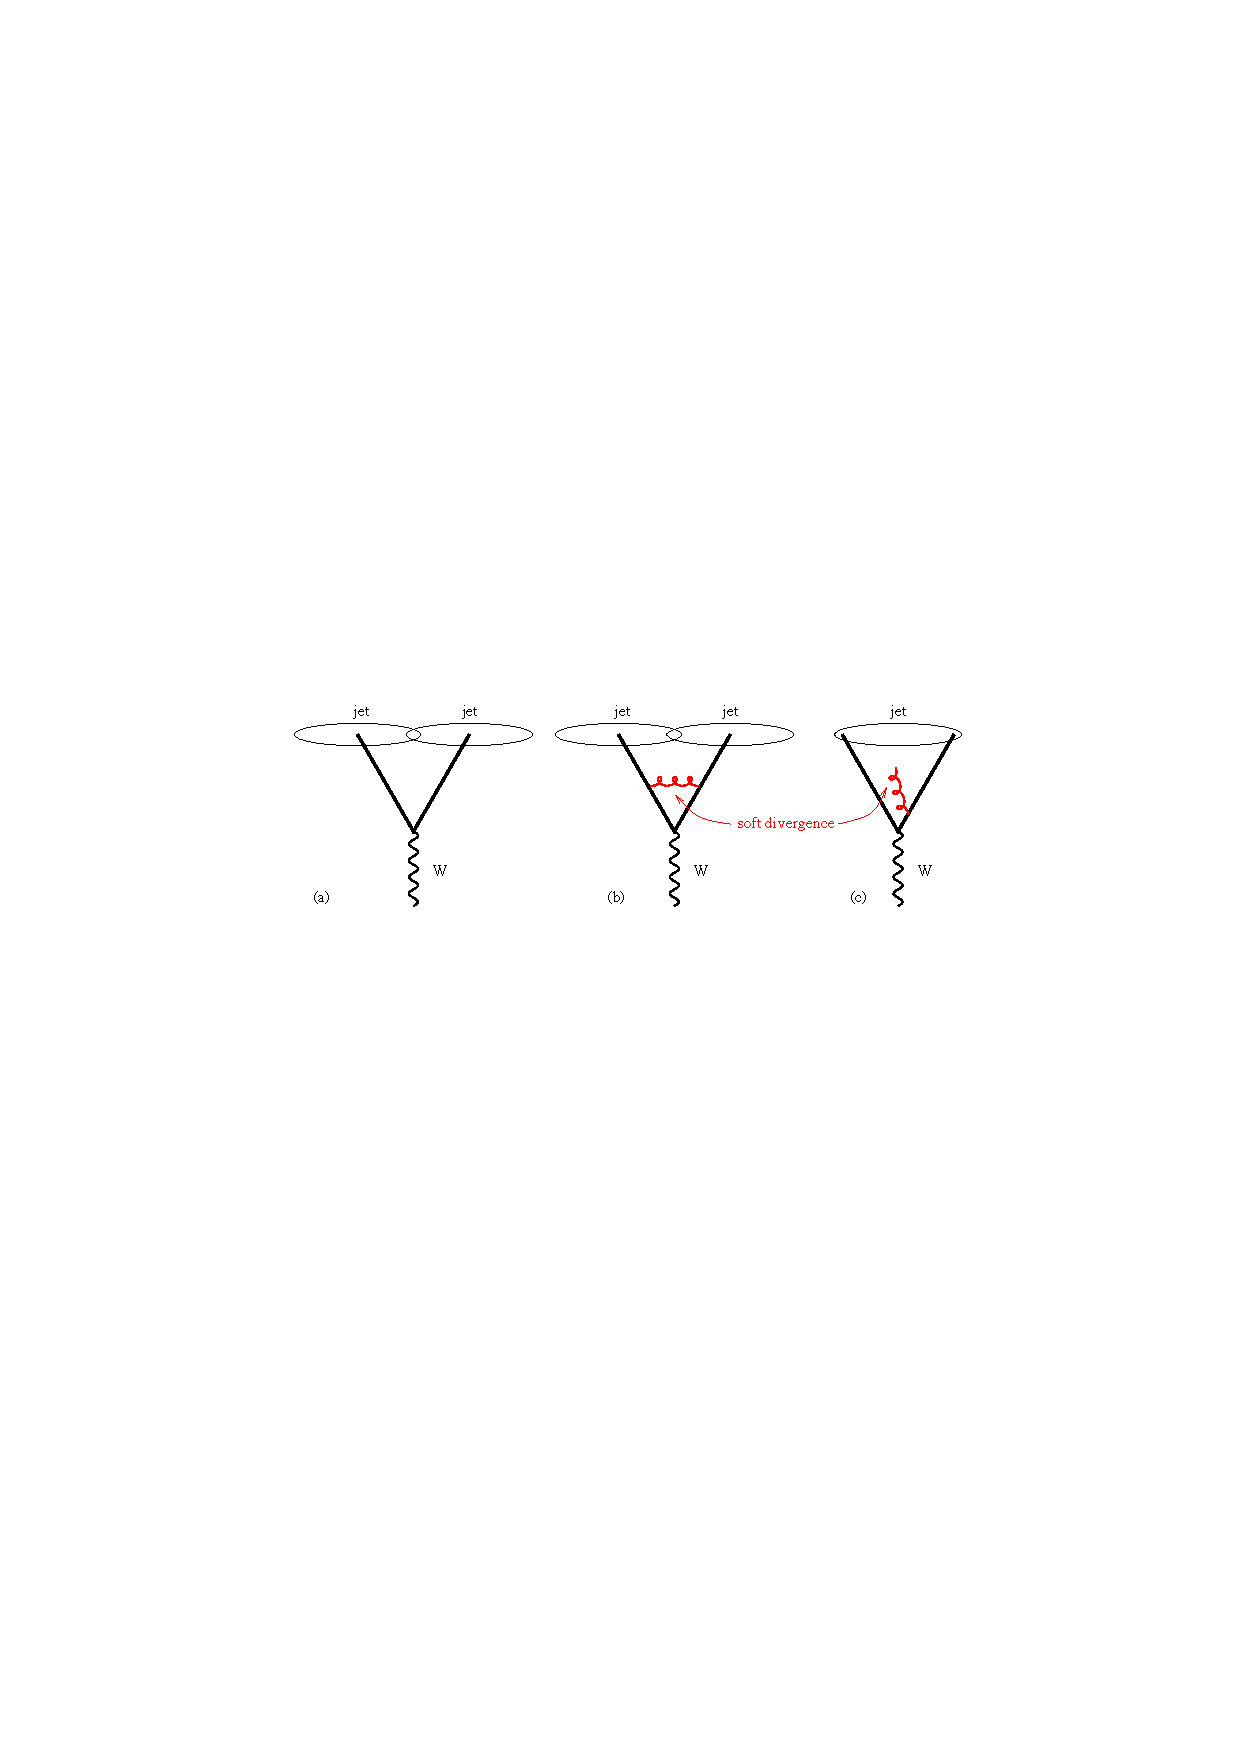
\includegraphics[width=0.8\textwidth]{Figures/jet_unsafe2.pdf}
		%\rule{35em}{0.5pt}
	\caption[An example of configuration of IRC unsafe jet algorithm.]{Configuration showing IC  unsafety with W boson and two partons. Adding a soft gluon causes two jets to be reconstructed as one. \cite{Salam:2009jx}}
	\label{fig:jet_unsafe}
\end{figure}

\par There are two types of jet algorithms which are most commonly used: \textit{cone algorithms} and \textit{sequential recombination algorithms}. In the case of \textit{cone algorithms}, a jet is defined as a set of particles inside a stable cone around their center of mass. Most popular cone algorithm is \textit{iterative cones} (IC) where a seed particle is chosen and momenta of all particles around that initial particle inside a cone of radius $R$ are summed. After adding each new particle to the sum, the direction of the new sum is taken as a seed direction, and the procedure repeats until the direction of the resulting cone is stable. Particles inside the cone are than removed from the list of available particles and the procedure repeats. This approach is not IRC safe given that nearly collinear splitting of the hardest particle in the event can be reconstructed as two jets. In that case, a less energetic, particle, pointing in another direction, can become the hardest particle in the event, yielding different set of jets. Cone algorithms can be IRC safe using a \textit{seedless cone} (SC) algorithm where all stable cone solutions are identified at once. However this approach is very time consuming even for small number of particles and thus very impractical to use.
In the \textit{sequential recombination algorithms} at hadron colliders two longitudinally invariant distances are introduced: $d_{ij}$ which is the distance between each pair of particles and $d_{iB}$ which is the particle-beam distance. These distances are defined as: 
\begin{equation}
d_{ij} = min(k_{T,i}^{2p},k_{T,j}^{2p}) \frac{\Delta R_{ij}^2}{R^2}
\end{equation}
\begin{equation}
d_{iB}=k_{T,i}^{2p}
\end{equation}
where $\Delta R_{ij}$ denotes the distance in the $\eta -\phi$ plane and is computed as $$\Delta R_{ij}^2 = (\eta_i-\eta_j)^2+(\phi_i-\phi_j)^2.$$ $k_T$ is transverse momentum of the particle, $R$ is an angular cut-off similar to the one in \textit{cone algorithms},  and $p$ defines which particles are clustered first and is described below. Both $R$ and $p$ are free parameters of the algorithm. The algorithm is applied using the following approach: distances $d_{ij}$ between each pair of particles, and $d_iB$ for each particle are computed and minimal value is found. If $d_{ij}$ is the smallest value, particles $i$ and $j$ are combined, and treated as a new particle in the next iteration of the algorithm. In case of $d_{iB}$ being the smallest, $i$ is declared to be the final jet and is removed from the list of particles. The procedure continues until there are no more particles in the list.
\begin{figure}[htbp]
	\centering
		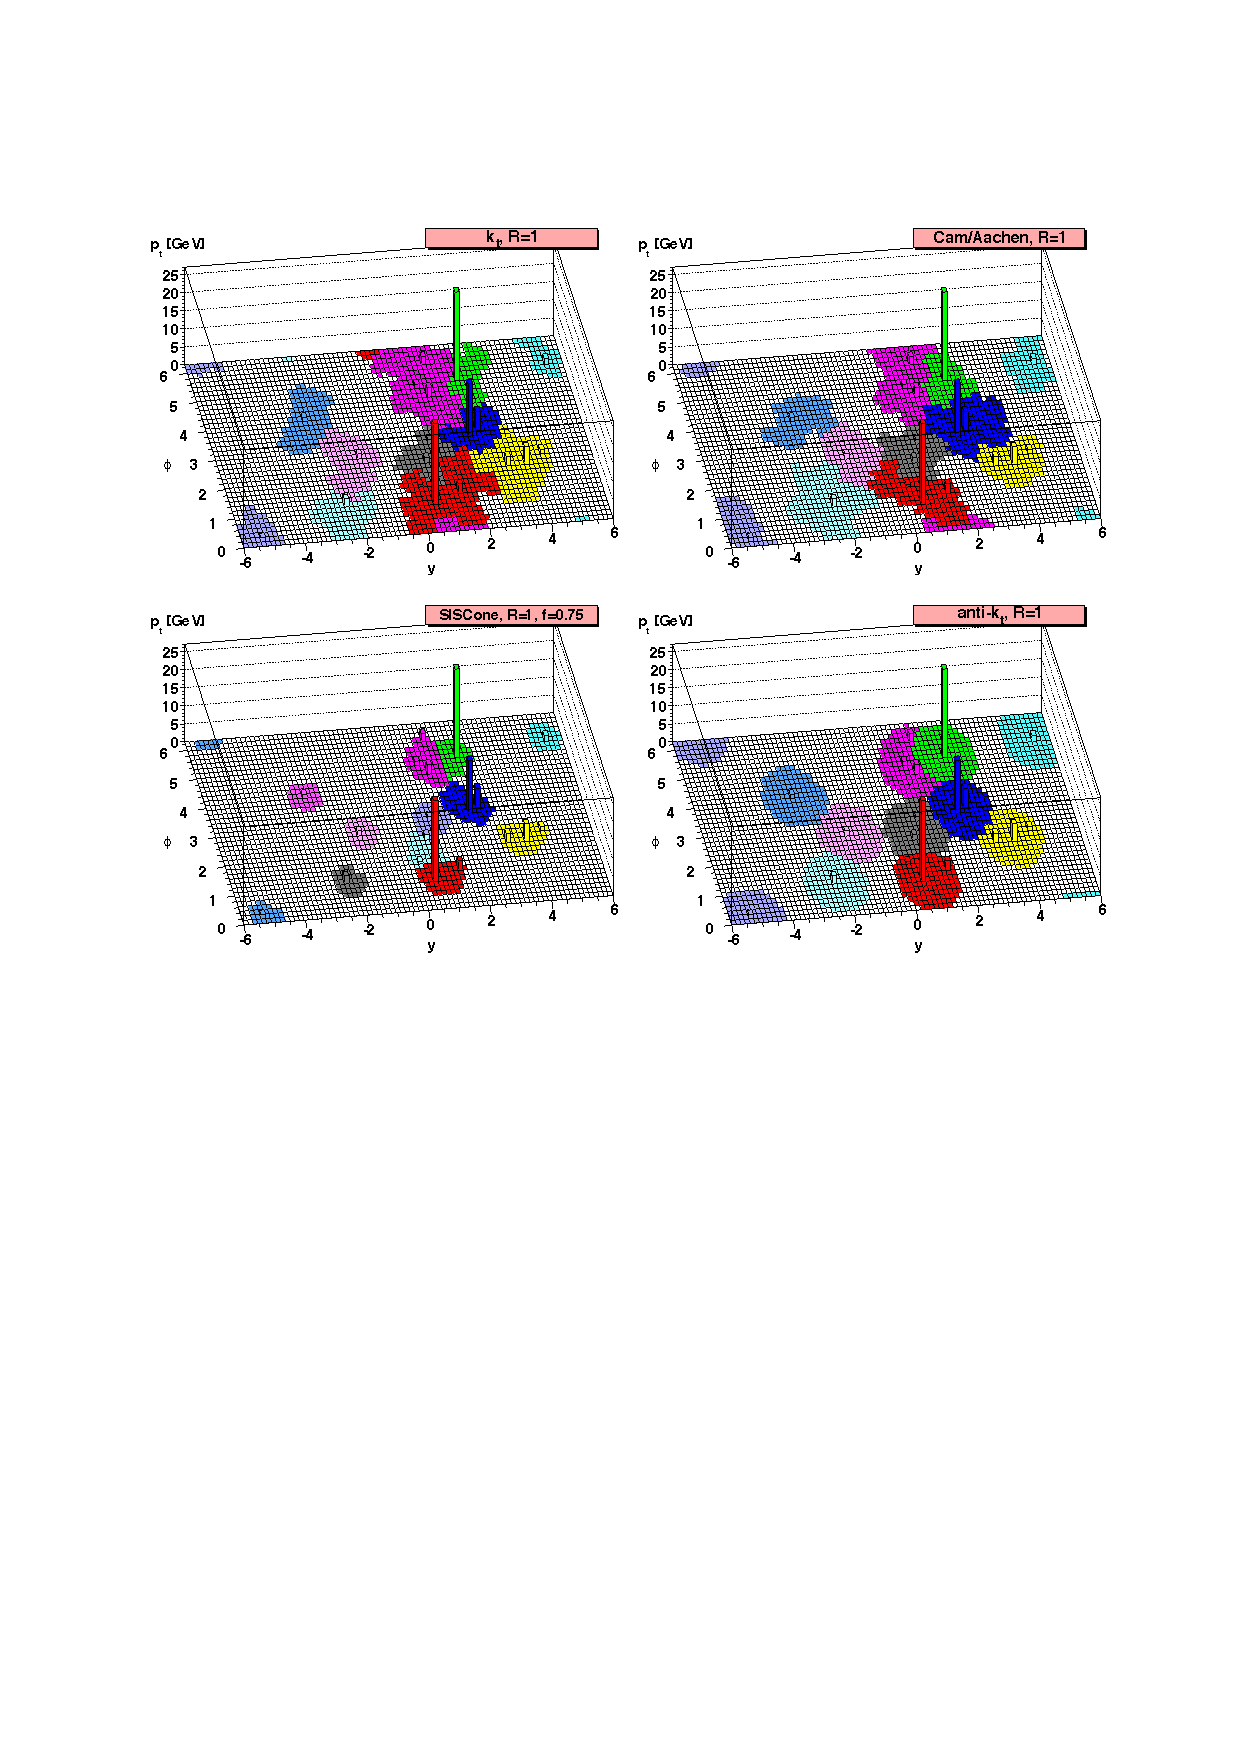
\includegraphics[width=0.9\textwidth]{Figures/diff_algos.pdf}
		%\rule{35em}{0.5pt}
	\caption[Clustering particles into jets with different algorithms.]{Clustering same set of reconstructed particles into jets using different jet algorithms. \cite{Salam:2009jx}}
	\label{fig:jetAlgos}
\end{figure}
\par The parameter $p$ defines which particles are clustered first thus defining the type of algorithm. The $k_T$ algorithm uses $p=1$, clustering soft particles first. This results in irregularly shaped jets, as shown in figure \ref{fig:jetAlgos}, which are sensitive to radiation in the event and difficult to calibrate. The \textit{Cambridge-Aachen} algorithm (CA) uses $p=0$ thus relying only on angular distribution of the input particles. This approach is particularly useful for jet substructure analysis and is less sensitive to radiation. The algorithm used in this analysis is anti-$k_T$ algorithm where $p=-1$ clusterizing the hardest particles first \cite{Cacciari:2008gp}. Anti-$k_T$ is an IRC safe algorithm and results with jets that are circular in shape because they are not affected by the softer components of the jet.       


%-----------------------------------
%	SUBSECTION 3.2
%-----------------------------------

\subsection{Jet corrections}
\label{sec:jetCorr}

Various measurements during the commissioning phase of the CMS detector showed that measured jet energy at detector level in general doesn't correspond to the energy of the originating particle. A jet calibration procedure is introduced to compensate for the nonlinear response of the calorimeters. This is done using a factorized approach where corrections on each level of correction are determined separately as described in \cite{Chatrchyan:2011ds}. The final corrected jet momentum is obtained from measured uncorrected transverse momentum $p^{raw}$ according to:
\begin{equation}
p^{corr} =  C_{res}(p_T'',\eta)\times  C_{abs}(p'_T) \times C_{rel}(\eta) \times C_{offset}(p_T^{raw},\eta)\times p^{raw}
\end{equation}  
Correction factors correspond to the following:
\begin{itemize}
\item The offset correction $C_{offset}$ compensates for energy contributions arising from pile-up events or instrumental noise. The offset is determined in dependence of pseudorapidity and jet area $p_T$ density which is described in detail in \cite{Cacciari2008119}.
\item The relative correction $C_{rel}$ aims at flattening the jet energy scale in pseudorapidity. The correction is determined from simulated QCD multijet events, adjusting the jet scale in all $\eta$ regions to one of the jets in $|\eta|<1.3$ without changing the absolute scale.
\item Absolute correction $C_{abs}$ flattens the jet scale in $p_T$. This correction is also determined from QCD multijet events as the inverse of average response at some fixed generated jet transverse momentum.
\item The residual correction $C_{res}$ is applied only to data in order to account for possible residual differences between data and simulation after applying absolute and relative corrections. These corrections are derived using events with momentum balance in the transverse plane, like dijet events or $Z/\gamma$ + jet events.
\end{itemize}   
$C_{offset}$ and calibration factors $C_{rel}$ and $C_{abs}$ are applied to both data and simulation and $C_{res}$ is applied only to data. Corrections are applied sequentially, in a fixed order such that $p_T' = C_{offset} \times C_{rel}(\eta) \times p^{raw}$ , and $p_T'' = C_{abs}(p'_T) \times C_{rel}(\eta) \times C_{offset}(p_T^{raw},\eta)\times p^{raw}$. Correction factors used in this analysis can be found in \cite{CMS-DP-2013-033}.
\par The total jet correction for a fixed jet $p_T$ as a function of pseudorapidity is shown in figure \ref{fig:tot_corr_eta}. The total jet correction for a fixed jet pseudorapidity as a function of transverse momentum is shown in figure \ref{fig:tot_corr_pt}. It is shown that jet energy correction factors for PF jets and JPT jets are relatively stable between 1 and 1.2 across wide $p_T$ and $\eta$ range. The total uncertainties to the jet energy corrections as a function of jet transverse momentum are shown in figure \ref{fig:tot_corr_err}.
\begin{figure}[htbp]
	\centering
		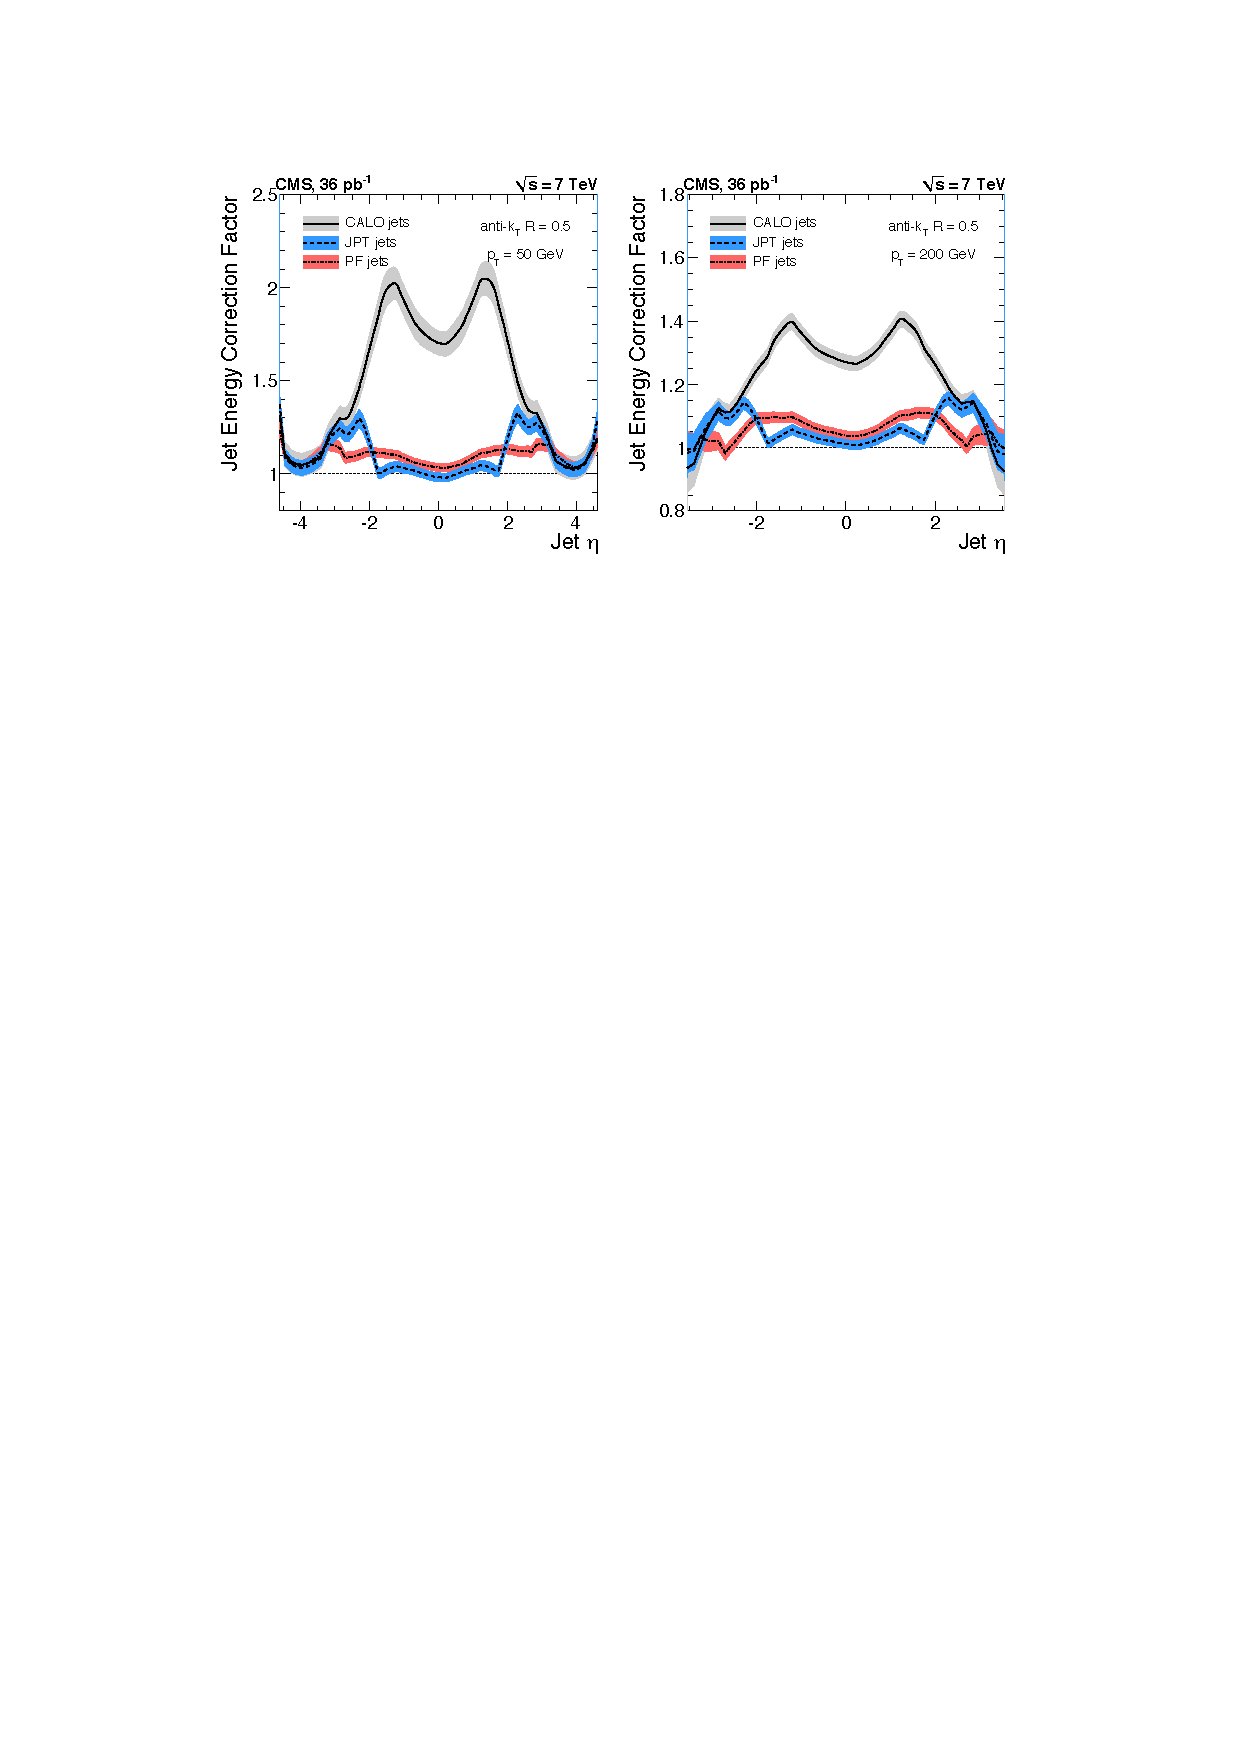
\includegraphics[width=0.9\textwidth]{Figures/jet_tot_corr_eta.pdf}
		%\rule{35em}{0.5pt}
	\caption[Total jet energy correction as a function of pseudorapidity of two different jet $p_T$ values.]{Total jet energy correction as a function of pseudorapidity of two different jet $p_T$ values. Corrections are shown for all three types of jets, calo, JPT and PF jets. Bands indicate corresponding uncertainty.\cite{Chatrchyan:2011ds}}
	\label{fig:tot_corr_eta}
\end{figure}

\begin{figure}[htbp]
	\centering
		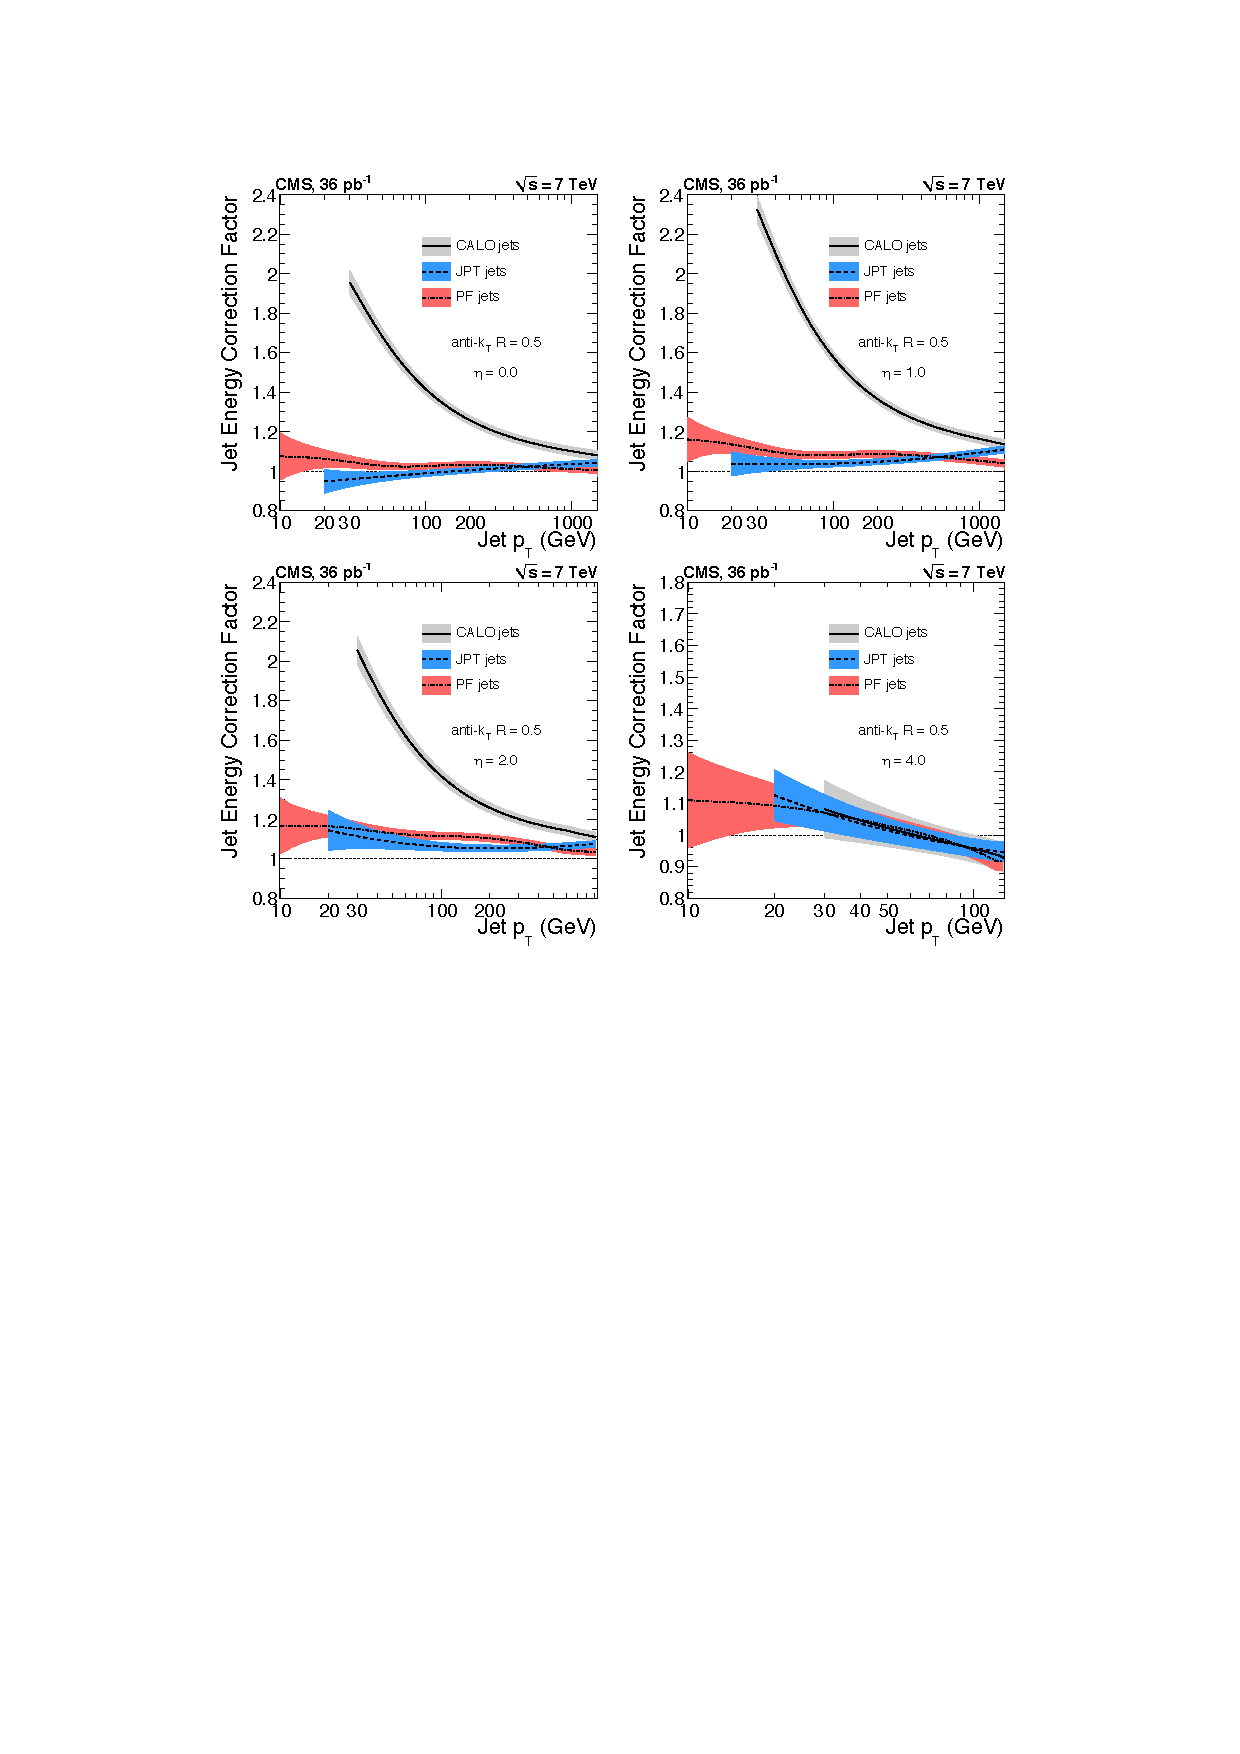
\includegraphics[width=0.9\textwidth]{Figures/jet_tot_corr_pt.pdf}
		%\rule{35em}{0.5pt}
	\caption[Total jet energy correction as a function of transverse momentum for four different $\eta$ values.]{Total jet energy correction as a function of transverse momentum for four different $\eta$ values. Corrections are shown for all three types of jets, calo, JPT and PF jets. Bands indicate corresponding uncertainty.\cite{Chatrchyan:2011ds}}
	\label{fig:tot_corr_pt}
\end{figure}

\begin{figure}[htbp]
	\centering
		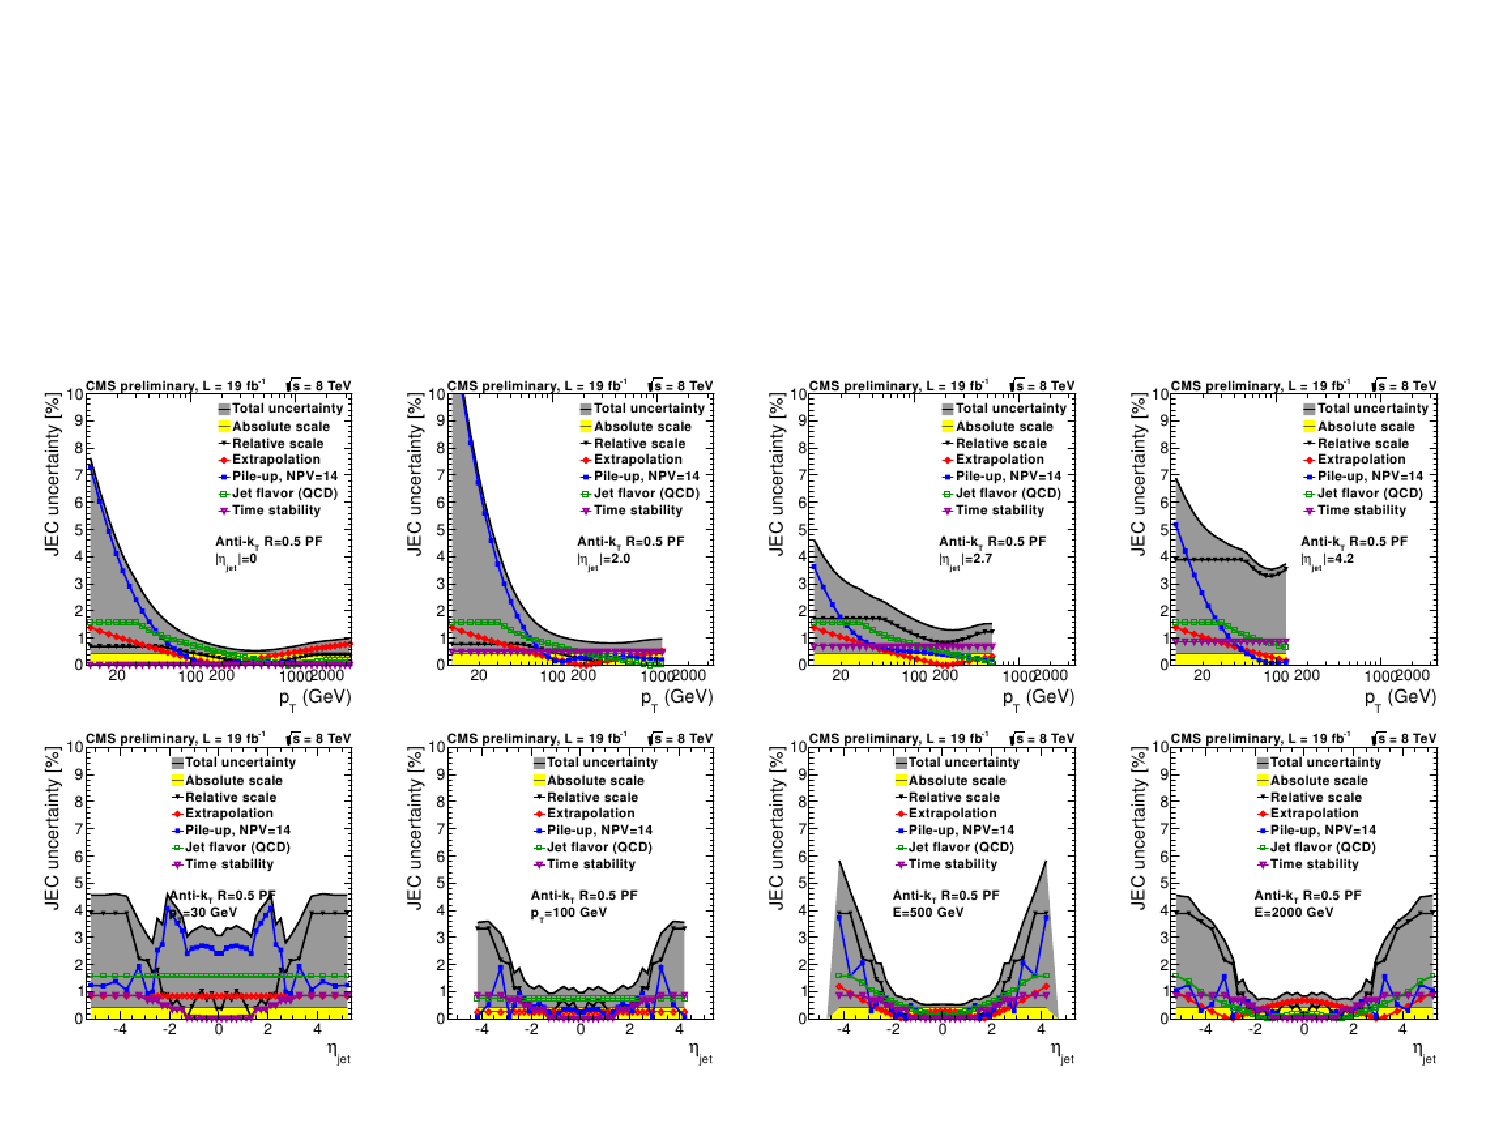
\includegraphics[width=0.9\textwidth]{Figures/jet_unc_err.pdf}
		%\rule{35em}{0.5pt}
	\caption{Total jet uncertainty and contribution from different sources in jet $p_T$ and $\eta$ \cite{CMS-DP-2013-033}}
	\label{fig:tot_corr_err}
\end{figure}

%-----------------------------------
%	SUBSECTION 3.3
%-----------------------------------

\subsection{Jet identification}
\label{sec:jetID}
This analysis uses the anti-$k_T$ algorithm with cone size $R=0.5$. Jet algorithm implementation is done in the FASTJET package \cite{Cacciari:2011ma}. Depending on which signals the algorithm is applied to, there are different kinds of jets: calo jets (calorimeter deposits used), jet-plus-track jets (calorimeter deposits complemented with tracker information) and most widely used \textit{particle flow} jets (PF). These jets are clustered from particle flow objects identified with the PF algorithm, thus using the information not only from HCAL, but also from the tracking system and ECAL, which result in much better resolution. Only the neutral fraction of  jets is measured with HCAL alone which makes about 15$\%$ of the total jet composition. PF jets show excellent performance and are the default jets for most CMS analyses. Pile-up information is also taken into account by removing charged hadrons originating from pile-up vertices from the list of particles available for the jet clusterization. This procedure is called \textit{charged hadron subtraction}. Some additional cuts to the jet composition are applied in order to ensure good jet identification. All jet identification criteria are summarized in the table \ref{tab:jetID}.  
  \begin{table}[h]
\centering
  \caption{A summary of jet identification criteria.}
  \label{tab:jetID}
  \begin{tabular}{ l  c c}
      \hline
      \hline
      	Variable & Requirement \\
      	\hline
    		Neutral hadron fraction & $<$ 0.99  \\
     	Neutral EM fraction & $<$ 0.99 \\
     	Number of Constituents & $>$ 1 \\		
		\hline
		Additional cuts for $|\eta|<2.4$ \\
		\hline
		Charged hadron fraction & $>$ 0 \\ 
		Charged multiplicity & $>$ 0 \\
		Charged EM fraction & $<$ 0.99 \\
      \hline
      \hline 
  \end{tabular}
\end{table}

%-----------------------------------
%	SUBSECTION 3.4
%-----------------------------------

\subsection{Jets from b quarks}
\label{sec:btagging}

The unique properties of the bottom quark can be used to identify hadronic jets originating from b quarks, which are usually referred to as b-jets. The long lifetime of B hadrons is a consequence of weak force decay which results in the displacement of their decay vertices by few millimeters at the LHC energies. These hadrons have relatively large masses and daughter particles with hard momentum spectra. The process of b-jet identification is called $b-tagging$. It takes one or more variables and produces a single discriminant value for each jet. This value shows how much the observed jet looks like a b-jet. There are several \textit{b-tagging} algorithms in use at CMS which are described in detail in \cite{Chatrchyan:2012jua} the following were used for 2012 data:
\begin{itemize}
	\item \textit{Track counting}(TC) - The discriminant uses the impact parameter significance, which is calculated as the impact parameter value divided by the respective impact parameter uncertainty. Impact parameter significance values are sorted in increasing order and the second or the third lowest value is used as a discriminant. Depending on whether the second or third value is chosen, the algorithm is denoted as high efficiency or high purity. 
	\item \textit{Jet Probability}(JP) - This algorithm combines information from several tracks inside a jet by computing a likelihood that all tracks originate from the primary vertex.  
	\item \textit{Combined secondary vertex}(CSV) - This is the most efficient \textit{b-tagging} algorithm currently used in CMS. Secondary vertex and track related informations are combined to build the CSV discriminator. It shows high efficiency even when no good secondary vertex can be reconstructed. Some of the variables used in the CSV algorithm are flight distance, vertex mass, impact parameter significance, track multiplicity at the vertex and track multiplicity in a jet. The distribution of CSV discriminator is shown in figure \ref{fig:csv}.
\end{itemize}
\begin{figure}[ht]
	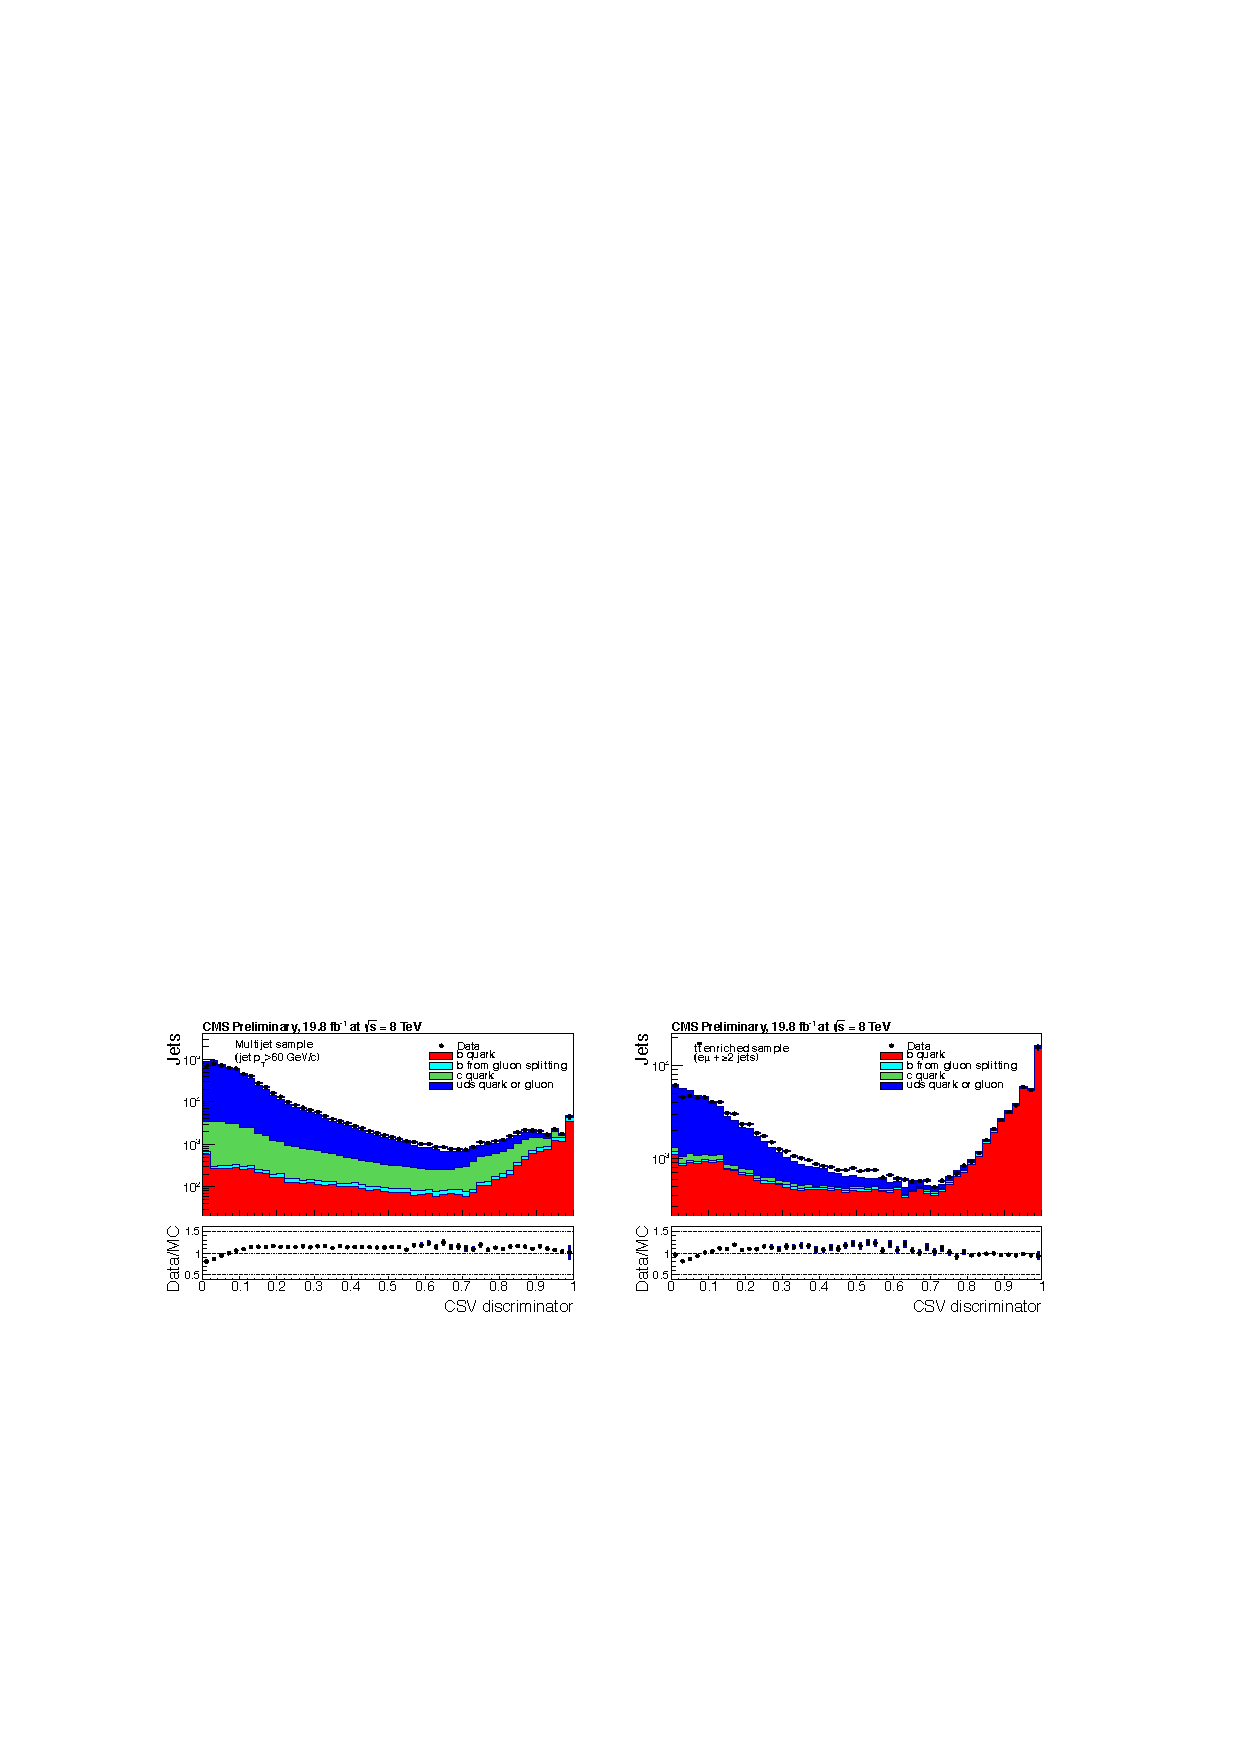
\includegraphics[width=\textwidth]{Figures/b-tag_csv.pdf}
	\caption{Combined secondary vertex discriminator for multijet QCD sample (left) and tt enriched sample(right)\cite{CMS:2013vea}}
	\label{fig:csv}
\end{figure}
For each non-b-jet there is a chance that it would be identified as b-jet. Three working points are chosen based on the mistagging efficiency. For an average jet of 80 GeV, these values correspond to misidentification rates of 10\%, 1\% and 0.1\%  for loose, medium and tight working point respectively \cite{1748-0221-8-04-P04013}. Misidentification probabilities as a function of b-jet transverse momentum for combines secondary vertex algorithm is shown in figure \ref{fig:misID}. 
\begin{figure}[ht]
\centering
	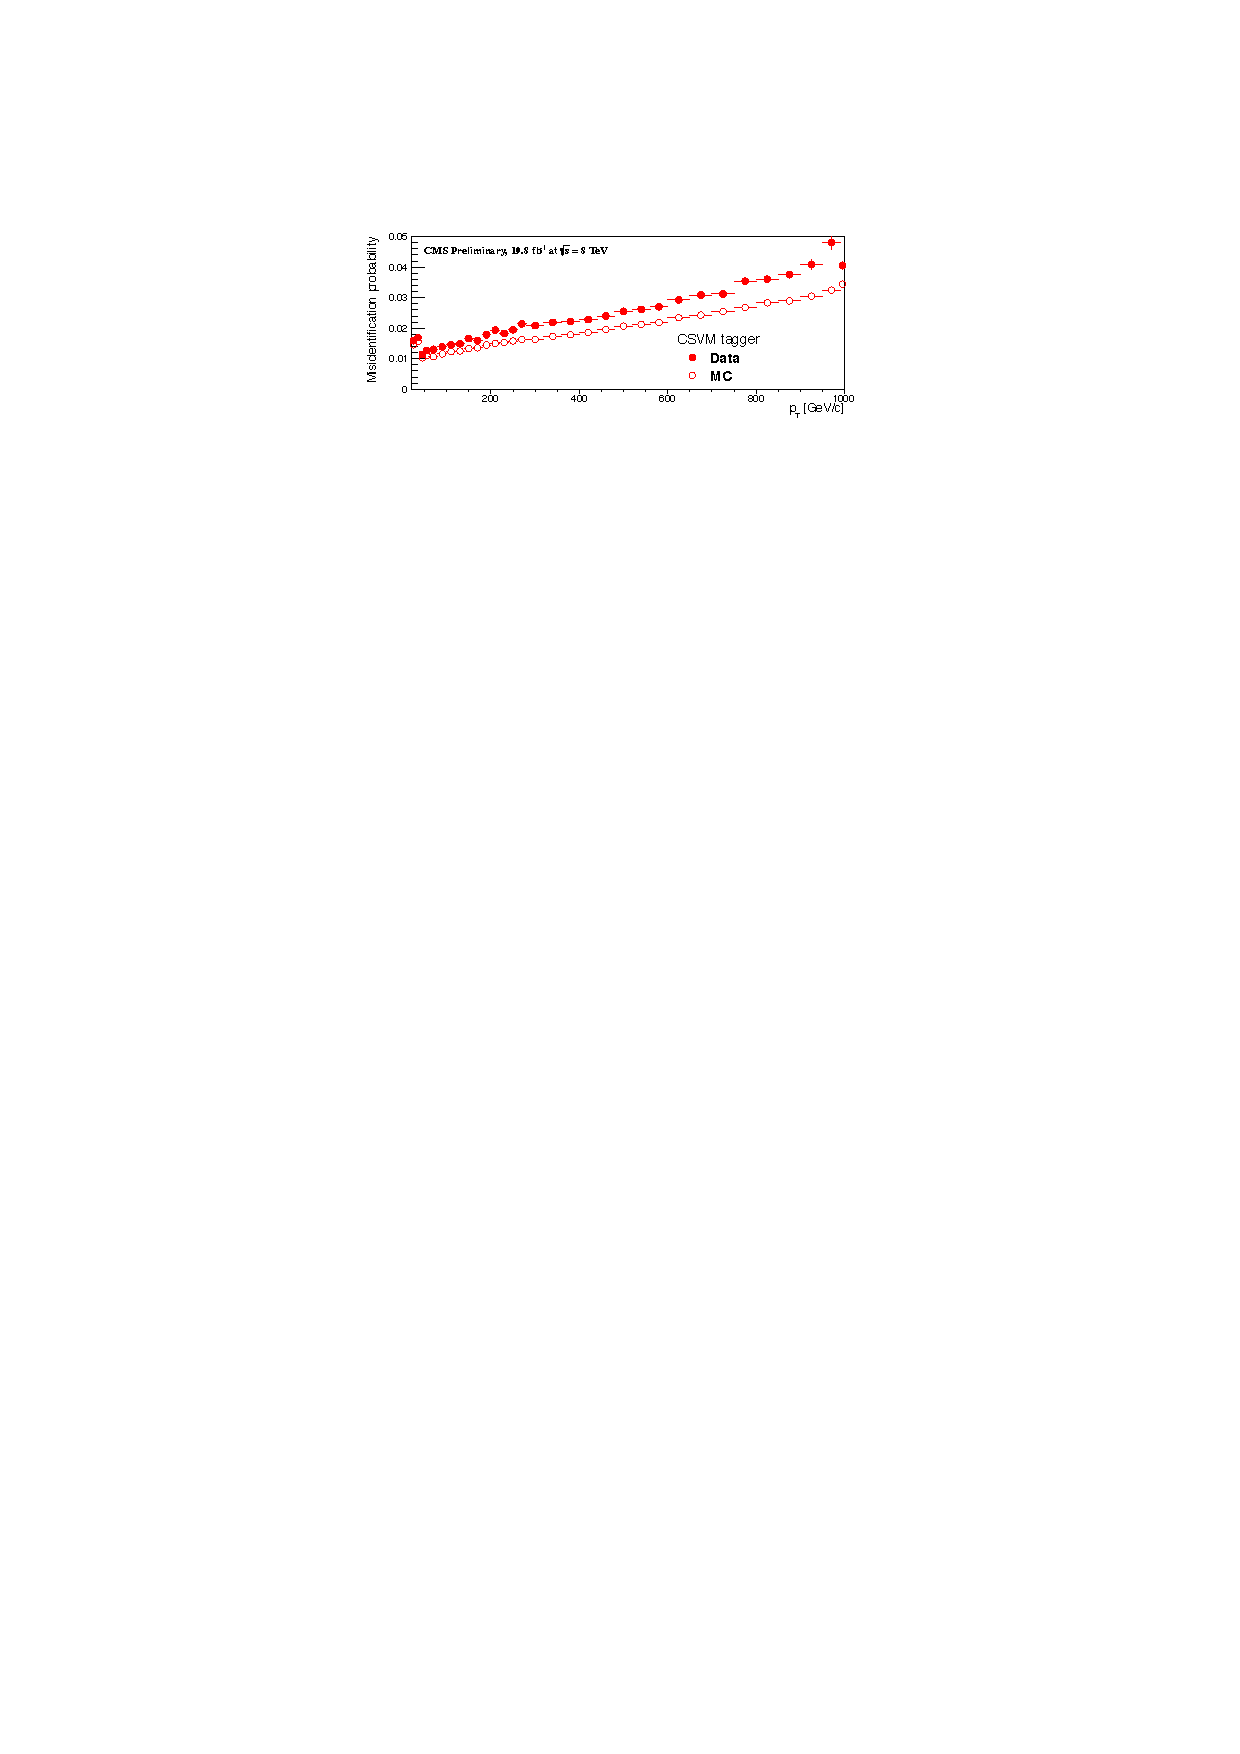
\includegraphics[width=0.6\textwidth]{Figures/MisID_CSVM.pdf}
	\caption{Combined secondary vertex misidentification probability for data and MC for medium working point.\cite{CMS:2013vea}}
	\label{fig:misID}
\end{figure}



%----------------------------------------------------------------------------------------
%	SECTION 4
%----------------------------------------------------------------------------------------

\section{Missing transverse energy}

The missing transverse momentum is the imbalance in the vectorial sum of transverse momenta of all measured particles. Missing transverse energy is the magnitude of the missing transverse momentum and is calculated as:
\begin{equation}
E_T^{miss}= |-\sum_{i} \vec{p}_i|
\end{equation}
where $i$ goes over all visible particles. Momentum conservation suggests that the imbalance could arise from weakly interacting neutral particles such as neutrinos or any other particle that doesn't interact with the detector. Measurement of the missing transverse energy relies on the good measurement of all other particles in the event and as such is very sensitive to detector resolution, particle missmeasurements, limited acceptance of the detector, cosmic-ray particles, all of which can cause artificial missing energy. There are several approaches to determine $E_T^{miss}$. In this analysis, the particle flow technique is used, which tries to identify each particle in the event by combining the information from all subdetectors and gives the best missing energy resolution.\cite{CMS-PAS-PFT-09-001,Chatrchyan:2011tn} Several corrections are applied to the $E_T^{miss}$ which correct for the possible bias in the missing energy measurement:
\begin{itemize}
\item Type-I correction: propagates jet energy corrections described in Section \ref{sec:jetCorr} to missing energy. This correction replaces the uncorrected transverse momenta of particles in a jet by the transverse momentum of a jet to which JEC were applied in the missing energy calculation.
\item xy-shift correction: aims at correcting the observed missing energy $\phi$ modulation. The true missing energy distribution is expected not to depend on $\phi$ because of the rotational symmetry of collisions around the beam axis. The possible causes for such modulation  include unisotropic detector response, detector misalignment or the displacement of the beam spot. The amplitude of the modulation is observed to increase with the number of pile-up interactions. This correction can thus be seen as mitigation for the pile-up effects.
\end{itemize}
Missing transverse energy, together with the reconstructed muon or electron, is used to construct W boson candidates. Transverse mass distribution particularly useful in the case of a decay into two particles, when one particle cannot be detected directly but is only indicated by missing transverse energy. If the daughter particles are massless, transverse mass is described with:   
\begin{equation}
M_T=\sqrt{2p_T^{lepton}E_T^{miss}(1-cos\Delta \phi)}.
\end{equation}



